\section{Verwendete Eingabegeräte \& Bibliotheken}
\label{hardware}
 wurden verschiedenen Farbkameras eingesetzt.\\
\\
%\subsection{Auswirkung von Pixelrauschen}
%Durch Aufnahme eines Schwarzbildes der Actioncam zeigt sich, dass das Pixelrauschen recht hoch ist, siehe \autoref{img_noishight}. Das Rauschen hat keine Normalverteilung, sondern es besteht aus kleinen Bereiche, die den selben fehlerhaften Farbwert besitzen.
%\begin{figure}
%	\centering
%	\fbox{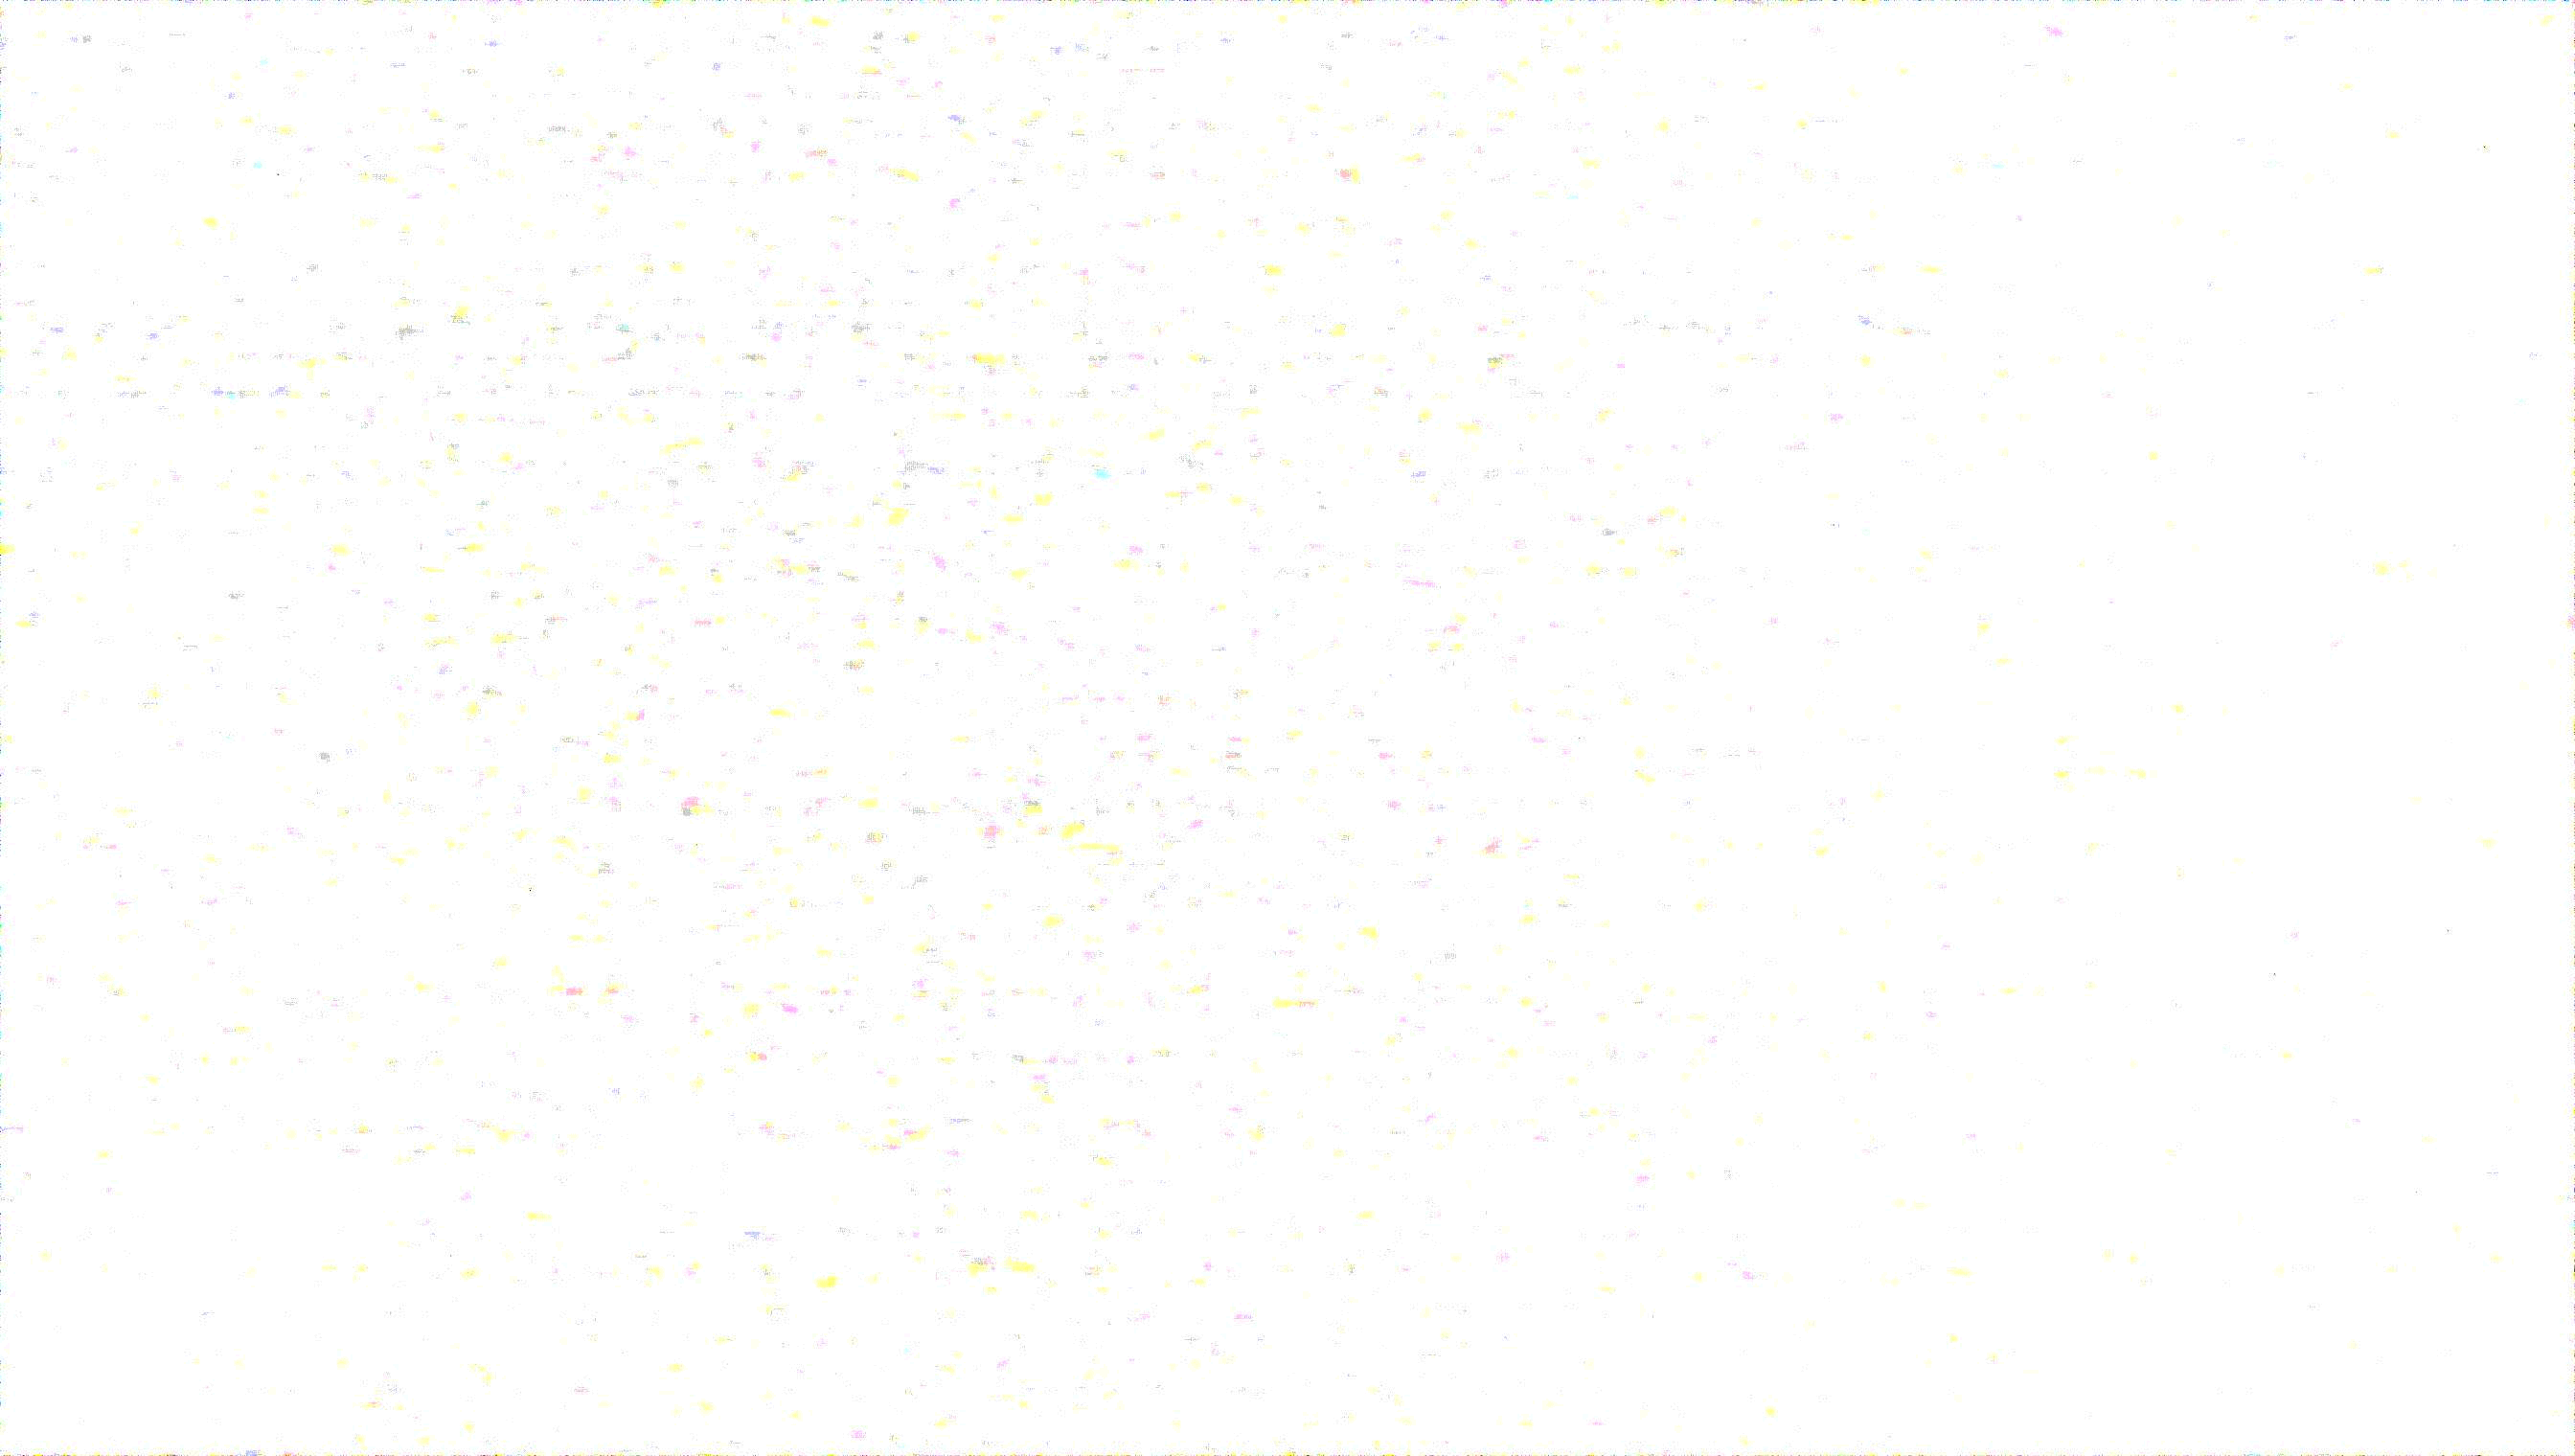
\includegraphics[width=1\linewidth]{img/NoisHight}}
%	\caption{Aufnahme eines Schwarz-Bildes $(2688\times 1520)$ der Actioncam um den Faktor 7 verstärkt und invertiert.}
%	\label{img_noishight}
%\end{figure}
Für die Umsetzung wurden Open Source Computer Vision (OpenCV 3.1) verwendet. Dies ist eine C/C++ Bibliothek von Algorithmen zur Bildverarbeitung in Echtzeit, veröffentlicht unter der BSD Lizenz (Berkeley
Software Distribution)\\
\cite{OpenCv_What_Is}\cite{wiki_Wha_is_OPenCV}